\section{Background and Motivation}

\subsection{Background}

\subsubsection{Streaming Graph Processing}

A graph $G=(V,E)$ consists of vertices $V$ and edges $E$. Algorithms such as breadth-first search (BFS), single-source shortest paths (SSSP), and connected components (CC) can be expressed as iterative worklist processing: active vertices update their neighbors and generate subsequent worklists until convergence~\cite{2013-Ligra}. In streaming graph processing, topology changes are commonly grouped into batches of edge insertions and deletions. Applying a batch $\Delta G_t$ transforms $G_t$ into $G_{t+1}$, whose analytical result is $R_{t+1}=\mathcal{A}(G_{t+1})$. Recomputing this result from scratch after each batch may repeat substantial work on unchanged graph regions.

\subsubsection{Streaming Graph Representation}
Streaming graph representations balance update efficiency, traversal locality, and memory overhead. Adjacency-list-based layouts organize neighbors separately for each vertex, enabling localized updates but potentially introducing fragmentation and indirection. CSR instead stores adjacency data contiguously using vertex offsets, providing compact storage and efficient traversal, while topology updates may require costly data movement. Dynamic representations address this trade-off through hierarchical storage, reserved space, or buffered updates. For example, Terrace uses a hierarchical graph container~\cite{2021-Terrace}, Spruce adopts a compact multilevel structure~\cite{2024-Spruce}, and LSMGraph combines an update-friendly LSM-tree with multilevel CSR storage~\cite{2024-LSMGraph}. These designs provide different balances between update cost and neighborhood access efficiency.

%引用GASGraph还是pcsr？
A representative approach incorporates a packed memory array (PMA) into the graph representation~\cite{2017-GPMA,2018-pcsr}. It stores the adjacency of all sources in a single shared array interleaved with gaps, so that the neighbors of each source remain contiguous and an insertion can usually be absorbed by a nearby gap. The array is divided into segments organized as an implicit tree, and each level enforces lower and upper density thresholds. As illustrated in Fig.~\ref{fig:increment-compute}(c), an insertion shifts the entries between its position and the nearest gap; when a segment exceeds its density threshold, the entries of an enclosing range are redistributed (rebalancing), and when the whole array becomes full, it is doubled in size and all entries are redistributed (expansion).

\subsubsection{Incremental Processing}
Incremental processing reuses the results of the previous graph snapshot and propagates update-induced changes through the affected dependencies. KickStarter uses dependency tracking and trimming to repair invalidated results~\cite{2017-KickStarter}, while GraphBolt tracks dependencies across intermediate values to support incremental processing with synchronous semantics~\cite{2019-GraphBolt}. For monotonic algorithms such as BFS and SSSP, dependency-memoization records for each vertex the parent through which its result was obtained. A deletion invalidates the results of all vertices that depend on the deleted edge; each invalidated result must then be restored from the remaining incoming edges of the vertex. An insertion can only improve results, and the improvement is propagated along outgoing edges. Figs.~\ref{fig:increment-compute}(a)–(b) illustrate how incremental computation repairs results via dependencies when the graph topology changes.

\subsubsection{Out-of-Memory CPU--GPU Graph Processing}
Out-of-memory systems keep edge data in host memory and place vertex results, together with per-vertex adjacency descriptors that record the location and degree of each neighbor list, on the GPU. Adjacency is transferred either explicitly after the CPU compacts the active subgraph, as in Subway~\cite{2020-Subway}, or on demand through zero-copy access, where GPU threads read pinned host memory with fine-grained PCIe requests, as in EMOGI~\cite{2020-EMOGI}. Grapin extends this model to streaming graphs: it maintains the dynamic topology on the CPU, performs incremental computation on the GPU, and caches the adjacency of frequently accessed vertices in GPU memory as a hot subgraph~\cite{2025-Grapin}. CoIncGraph adopts this execution model, including zero-copy access and hotness-based subgraph caching.

\begin{figure}[t]
\centering
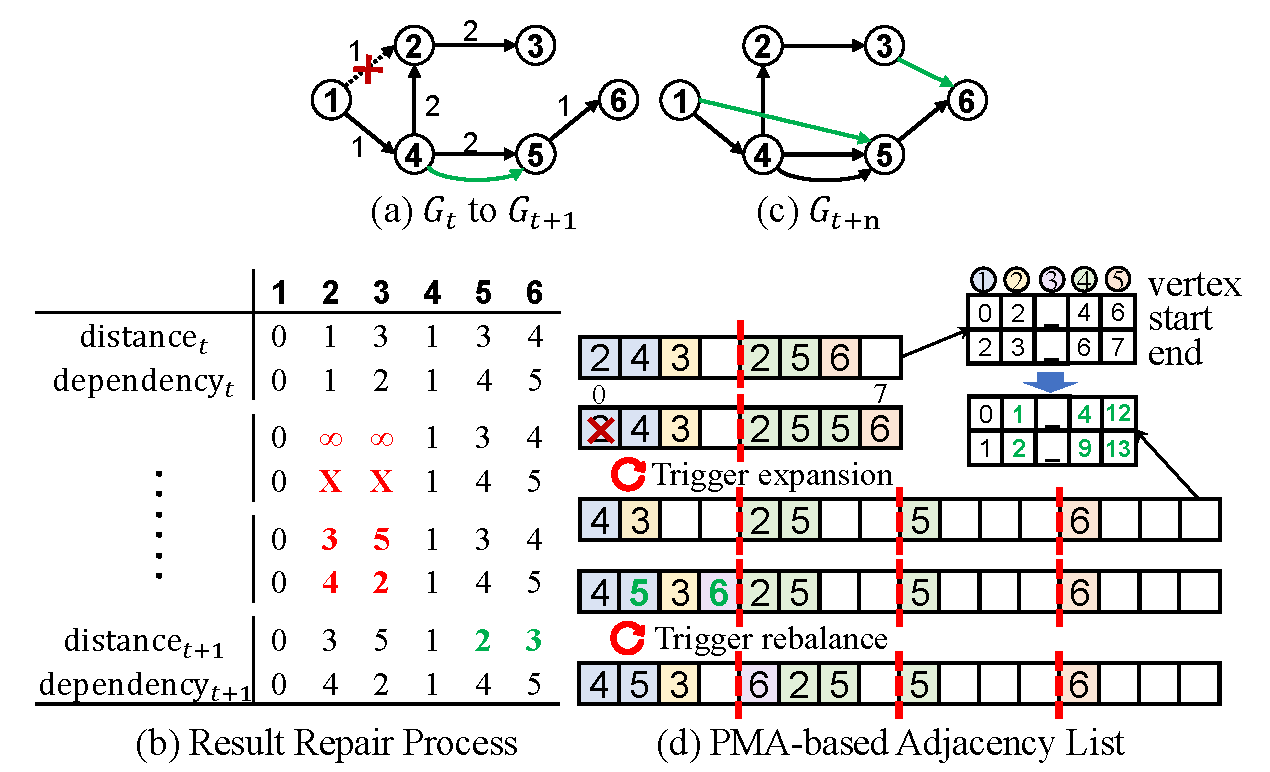
\includegraphics[width=\columnwidth]{figures/increment compute.pdf}
\caption{PMA-based adjacency maintenance and incremental result repair. (a)--(b) An edge update transforms $G_t$ into $G_{t+1}$ and propagates its effect to dependent vertices. (c) In the PMA, local shifts may change the indices of subsequent adjacency entries; insufficient local space triggers expansion, and density violations trigger rebalancing over a larger range. (d) The corresponding vertex results and dependencies are repaired to obtain the state for $G_{t+1}$.}
\label{fig:increment-compute}
\end{figure}

\subsection{Motivation}
\label{sec:motivation}

% 数据来源：paper/evaluation/raw/motivation_sssp_20261003/averages.csv（SSSP，TW/FS，100K，十批均值，counts/timing 各两次，Grapin=original）。
% Upd.=批内更新触及的源（去重）；Desc.=显式 H2D descriptor payload（MB=10^6 B；Grapin 约 16 B/顶点，CoIncGraph 约 24 B/源）；Init. WL=插入阶段初始 worklist 长度（CoIncGraph 即被插入边直接改善的终点数，与 seeds_prebatch 一致）。
% 未使用：Reloc.（Grapin 批边界净地址变化为 0）、|A|（Grapin 更小且两系统定义不同）、Rebuild 占比（5.3%/5.7%，说服力弱）、Seeds（与 CoIncGraph 的 Init. WL 重复）。
Out-of-memory streaming graph processing typically keeps the complete topology in host memory and places vertex results on the GPU, exploiting its high memory bandwidth and massive parallelism for computation, while adjacency is fetched from host memory over the PCIe bus on demand. Since PCIe bandwidth is far lower than device memory bandwidth, every adjacency transfer and every update to GPU-side graph views incurs substantial cost. Fortunately, streaming updates exhibit \textit{update locality}: in Twitter (TW) and Friendster (FS), a 100K-edge batch touches only 0.18\% and 0.15\% of the sources, respectively (Upd.\ in Table~\ref{tab:motivation}), so both costs should ideally scale with the changed region. However, we observe that existing designs lose this locality in both graph maintenance and incremental computation.

\begin{table}[t]
\centering
\caption{Per-batch statistics of SSSP (100K-edge batches, averaged over ten batches). Upd.: sources touched by the batch; Desc.: descriptor data transferred to the GPU; Init.\ WL: size of the initial insertion worklist.}
\label{tab:motivation}
\footnotesize
\setlength{\tabcolsep}{4pt}
\begin{tabular}{llrrr}
\hline
Graph & System & Upd. & Desc. (MB) & Init.\ WL \\
\hline
TW & Grapin~\cite{2025-Grapin} & 94,869 & 841.3 & 52,579,682 \\
 & CoIncGraph & 94,869 & 2.3 & 1,126 \\
\hline
FS & Grapin~\cite{2025-Grapin} & 99,188 & 1,049.7 & 65,608,366 \\
 & CoIncGraph & 99,188 & 2.4 & 1,684 \\
\hline
\end{tabular}
\end{table}

\textbf{Graph maintenance amplifies local updates.} Shared-array layouts, such as PMA or CSR, keep each source's adjacency contiguous for coalesced GPU access, but an insertion may shift, rebalance, or expand a range containing sources that receive no update. Since such relocations are decided inside the layout and cannot be derived from the update batch, publishing descriptors only for updated sources would risk leaving relocated sources pointing to stale locations; the descriptors of all $|V|$ vertices are therefore reloaded after every batch. As shown in Table~\ref{tab:motivation}, this transfers 841\,MB and 1,050\,MB of descriptors per batch in TW and FS, i.e., 16 bytes for every vertex, although fewer than 0.2\% of the sources are touched; publishing only the touched sources, as CoIncGraph does, reduces this volume to about 2\,MB. The GPU cache suffers similarly: modifying a cached source invalidates its cached adjacency, and the cache is evicted, compacted, and reloaded after every batch, even when the set of hot vertices barely changes. Consequently, maintenance cost scales with the graph rather than with the changed sources. This calls for a graph organization that confines relocation to updated sources, so that every CPU- and GPU-side graph view can be maintained at the granularity of changed sources.

\textbf{Incremental computation loses its affected region.} Restoring an invalidated vertex $v$ requires one of its remaining incoming edges, e.g., $(x,v)$, yet the predecessor $x$ is unaffected by the batch and thus inactive, and a GPU engine that traverses outgoing edges cannot locate it. Recovery is therefore merged into insertion processing, which reactivates all vertices and rebuilds worklists by scanning vertex states in every round~\cite{2025-Grapin}. As a result, the initial insertion worklist contains all 52.6M and 65.6M vertices in TW and FS, whereas only about 1.1K and 1.7K destinations are directly improved by inserted edges and need to start propagation, which is the initial worklist of CoIncGraph (Table~\ref{tab:motivation}). The missing incoming adjacency, however, is readily available on the CPU, which maintains the topology in host memory. If the CPU supplies the incoming edges of invalidated vertices, deletion repair can be completed within the affected region before insertions are applied, after which insertion propagation needs to start only from the improved vertices. This motivates decoupling deletion repair from insertion propagation through CPU--GPU cooperation and keeping worklists compact throughout. Sections~\ref{sec:graph-organization} and~\ref{sec:incremental-computation} present the designs that address these two observations.
